\DiaryEntry{Game Theory, Static Settings}{2023-11-21}{Game Theory}

We study rational behavior of all game participants. The tools treat strategies and payoffs as fundamental; that is, they address the normal-form specification of a game. Because extensive-form games can be easily translated into the normal form, the analysis developed here applies also to extensive-form representations. The theory here is best applied to games in which all of the players’ actions are taken simultaneously and independently; ie. one-shot, or static, games.

\subsection{Dominance}

As a motivating example, consider the following three games. In the game (a), strategy U has the property, that regardless of player 2’s choice, strategy U gives player 1 a strictly higher payoff than does D. If player 2 plays L, then player 1 obtains 2 from playing U and 1 from playing D. Obviously, U is better in this case. Furthermore, if player 2 selects R, then player 1 obtains 5 by playing U and 4 by playing D. Again, U is better.

Technically, we say that strategy D is \emph{dominated} by strategy U, and thus D should never be played by a rational player 1. Note that neither of player 2’s strategies is dominated. Strategy L is better than R if player 1 selects U, but the reverse is true if player 1 selects D.

As a second example, consider game (b): Player 1’s strategy D is dominated by strategy M. Regardless of what player 2 does, M yields a higher payoff for player 1 than does D. Strategy U is not dominated by M, however, because, if player 2 were to play L, then U would give player 1 a higher payoff than would M.

\begin{figure}[H]
    \centering
    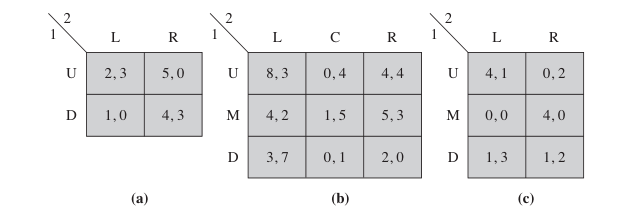
\includegraphics[scale=0.7]{images/2023-11-21-game_theory_01.png}
\end{figure}

Finally, game (c) is a bit more tricky: For player 1 no pure strategy is dominated by another pure strategy. Obviously, neither U nor M dominates the other, and D does not dominate these strategies. In addition, neither U nor M dominates D. For instance, although U is better than D when player 2 selects L, D performs better than U when player 2 selects R.

However, a \emph{mixed strategy} dominates D. Consider player 1’s mixed strategy of selecting U with probability $1/2$, M with probability $1/2$, and D with probability zero. We represent this mixed strategy as $(1/2, 1/2, 0)$. If player 2 selects L, then this mixed strategy yields an expected pay off for player 1 as follows,

\bee
u_1 = 4 \times \frac{1}{2} + 0 \times \frac{1}{2} + 1 \times 0 = 2,
\eee

which is better than the pure strategy D of player 1. If player 2 selects R, then we obtain an expected pay off for player 1 as,

\bee
u_1 = 0 \times \frac{1}{2} + 4 \times \frac{1}{2} + 1 \times 0 = 2,
\eee

and this is again better than D. Therefore, the mixed strategy $(1/2, 1/2, 0)$ dominates the pure strategy D for player 1.

We formally define dominance as follows.

\begin{definition}
A pure strategy $s_i$ of player $i$	is \emph{dominated} if there is a (pure or mixed) strategy $\sigma_i \in \Delta S_i$, such that

\bee
u_i(\sigma_i, s_{-i}) > u_i(s_i, s_{-i}), \quad \forall s_{-i} \in S_{-i}
\eee
\end{definition}

Note the importance of greater-than (and not greater or equal) in the payoff function comparison. 

The decision whether a strategy is dominated by another can be tricky, in particular when mixed strategies are considered.

A rational player will not chose a dominated strategy, as he could choose the dominating strategy to increase his payoff (and that's the definition of rational behaviour: Every player behaves in such a way as to maximize his payoff).

Note that there can be a clash between individual and group interests. As an example, consider the prisoner's dilemma described in Section \ref{2023-10-10:classicalgames}: For both players, strategy C is dominated by strategy D. Being rational, we would therefore predict that neither player would select C.

However, both players would be better off if they each selected C as they are jointly better off if they each select C rather than D. However, each has the individual incentive to defect by choosing D. Because the players select their strategies simultaneously and independently, individual incentives win.



\subsection{Best Response}

While strategy domination is an important concept, in most games, players have more than one undominated strategy: Matching pennies, the battle of the sexes, and the coordination games have no dominated strategies, so one cannot predict how people should or will play these games on the basis of the dominance criterion.

Rational players think about the actions that the other players might take; that is, people form beliefs about one another’s behavior and use these beliefs before deciding their own strategy. For example, in the coordination game, if player 1 thinks the other player will play strategy B, then he will also choose strategy B. 

In order to maximize payoff (which we assume is rational behaviour), every player selects the that yields the greatest expected payoff against the player's belief. Such a strategy is called a best response (or best reply).

\begin{definition}
	If a player $i$ has  a belief $\sigma_{-i} \in \Delta S_{-i}$ about the strategies played by the other players, then player $i$'s strategy $s_i \in S_i$ is a \emph{best response} if
	
	\bee
		u_i(s_i, \theta_{-i}) \geq u_i(s'_i, \theta_{-i}), \quad \forall s'_i \in S_i
	\eee
\end{definition}

Note that the best response depends on the belief about the other player's strategies.

The best response is illustrated with the following example.

\begin{figure}[H]
    \centering
    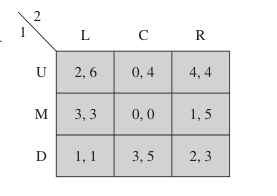
\includegraphics[scale=0.7]{images/2023-11-21-game_theory_02.png}
\end{figure}

Player 1's belief is that player 2 will choose L with probability $1/3$, C with probability $1/2$, and R with probability $1/6$. We can write this belief as $(1/3, 1/2, 1/6)$. Based on these beliefs, player 1 calculates the expected outcome for each of his strategies as

\begin{align*}
u_1(U, (1/3, 1/2, 1/6)) &= 2 \times \frac{1}{3} + 0 \times \frac{1}{2} + 4 \times \frac{1}{6} = \frac{8}{6} \\
u_1(M, (1/3, 1/2, 1/6)) &= 3 \times \frac{1}{3} + 0 \times \frac{1}{2} + 1 \times \frac{1}{6} = \frac{7}{6} \\
u_1(D, (1/3, 1/2, 1/6)) &= 1 \times \frac{1}{3} + 3 \times \frac{1}{2} + 2 \times \frac{1}{6} = \frac{13}{6}
\end{align*}

Therefore, player 1's best response is strategy D, the strategy that yields the greatest expected payoff given his belief. In addition, Strategy D is player 1's only best response,

\bee
BR_1 (1/3, 1/2, 1/6) = \{D\}.
\eee

Had player 1 different beliefs, the best response becomes different; eg for the belief $(1/6, 5/6, 0)$, the payoffs are

\begin{align*}
u_1(U, (1/6, 5/6, 0)) &= \frac{1}{3} \\
u_1(M, (1/6, 5/6, 0)) &= 1 \\
u_1(D, (1/6, 5/6, 0)) &= 1
\end{align*}

and therefore the best response consists of the two strategies

\bee
BR_1 (1/6, 5/6, 0) = \{M, D\}.
\eee


\subsection{Domaince and Best Response Compared}

not sure if we want to include it


 \subsection{Rationalizability and Iterated Dominance}
 
The concepts of dominance and best response form the basis of game theory; however, we can also put ourselves in the shoes of the other players for further insights into our optimal decision.

We illustrate this with the following example.

\begin{figure}[H]
    \centering
    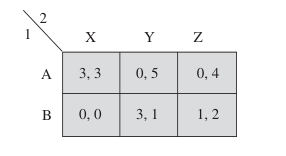
\includegraphics[scale=0.7]{images/2023-11-21-game_theory_03.png}
\end{figure}


We start our analysis by noting that both players are rational (and know this from each other). In addition, both players know the game; ie the matrix is known. Looking at the matrix, we see that no strategy is dominant for player 1; however, for player 2, strategy X is strictly dominated by Y. Therefore, player 2 will not play X. As a consequence, we can remove the matrix columncorresponding to strategy X, effectively leading to a new game as depicted in the following Figure (a). In this game, player 1 has strategies A and B, player 2 has strategies Y and Z. In this reduced game, player 1's strategy A is strictly dominated by strategy B; this allows us to remove the matrix row corresponding to strategy B, resulting in the new gane as shown in (b). We can continue with this approach and see that now for player 2, strategy Y is dominated by strategy Z. This leads to the "final" game with a $1 \times 1 $ matrix, where player 1 chooses strategy B and player 2 chooses strategy Z. The resulting payoff is then $(1,2)$.

\begin{figure}[H]
    \centering
    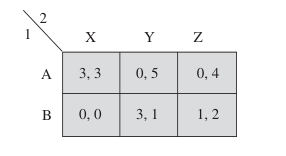
\includegraphics[scale=0.7]{images/2023-11-21-game_theory_03.png}
\end{figure}

Note that as in the prisoners’ dilemma, the prediction here is a decidedly inefficient outcome. Both players could fare better if the strategy profile
(A, X) were played, but neither player finds it in his or her interest to do so.

The procedure just illustrated is called \emph{iterative removal of (strictly) dominated strategies} (or iterated dominance, for short). We can apply the procedure to any normal-form game as follows. First, delete all of the dominated strategies for each player, because a rational player would never use one of these. Then define $R_1$ to be the strategy profiles that remain. Common knowledge of rationality therefore implies that it is common knowledge that a strategy profile in $R_1$ will be played. In other words, essentially the players are interacting in a “reduced” game in which $R_1$ is the set of strategy profiles. The next step is to remove any strategies that are dominated in this reduced game and define $R_2$ as the strategy profiles that remain. As before, it is then common knowledge that a strategy profile in $R_2$ will be played. Continue this process to identify smaller and smaller sets of strategy profiles, $R_3, R_4, \ldots$, until no more strategies can be deleted. Let $R$ denote the resulting set of strategy profiles; ie those that survive this iterated dominance procedure.




%%% Local Variables:
%%% mode: latex
%%% TeX-master: "journal"
%%% End:
